\documentclass[12pt]{article}  % 官方要求字号不小于 12 号,此处选择 12 号字体

% 本模板不需要填写年份,以当前电脑时间自动生成
% 请在以下的方括号中填写队伍控制号
\usepackage[UTF8]{ctex}
\usepackage{float}
\usepackage{algorithm}
\usepackage{algorithmic}
\usepackage[2510625]{easymcm}  % 载入 EasyMCM 模板文件
\problem{B}  % 请在此处填写题号
% \usepackage{mathptmx}  % 这是 Times 字体,中规中矩 
\usepackage{mathpazo}  % 这是 COMAP 官方杂志采用的更好看的 Palatino 字体,可替代以上的 mathptmx 宏包
\makeatletter
\newenvironment{breakablealgorithm}
  {% \begin{breakablealgorithm}
   \begin{center}
     \refstepcounter{algorithm}% New algorithm
     \hrule height.8pt depth0pt \kern2pt% \@fs@pre for \@fs@ruled
     \renewcommand{\caption}[2][\relax]{% Make a new \caption
       {\raggedright\textbf{\ALG@name~\thealgorithm} ##2\par}%
       \ifx\relax##1\relax % #1 is \relax
         \addcontentsline{loa}{algorithm}{\protect\numberline{\thealgorithm}##2}%
       \else % #1 is not \relax
         \addcontentsline{loa}{algorithm}{\protect\numberline{\thealgorithm}##1}%
       \fi
       \kern2pt\hrule\kern2pt
     }
  }{% \end{breakablealgorithm}
     \kern2pt\hrule\relax% \@fs@post for \@fs@ruled
   \end{center}
  }
\makeatother
\title{An MCM Paper Made by Team 2510625}  % 标题

% 如需要修改题头(默认为 MCM/ICM),请使用以下命令(此处修改为 MCM)
%\renewcommand{\contest}{MCM}

% 文档开始
\begin{document}

% 此处填写摘要内容
\begin{abstract}
    Here is the abstract of our paper.

    \textbf{For Problem1}, 通过数据分析,我们发现游客人数、税率和基建投入占比对收入有影响。为此,我们构建了一个综合收入、社会满意度和环境质量的目标函数,并采用多起点优化算法寻找最优解。基于朱诺市的历史数据,我们对社会满意度和游客人数进行了非线性拟合,拟合可靠度为0.7423。通过去量纲处理,我们量化了社会满意度和环境质量对目标函数的影响。
	模型结果显示,当游客人数为1,431,579人,游客税率为8\%,废物管理投入占比为0.179,水资源管理投入占比为0.113,环境保护投入占比为0.108时,总收入达到272亿美元,$\text{CO}_2$排放量为1,331,368.42吨,居民满意度为67.18(满分100),环境指数为0.4876(满分1,越小越好)。
	在敏感性分析中,我们评估了变量的局部和全局敏感性,发现游客人数是关键变量。最后,我们使用种群迭代算法和帕累托优化对模型进行了验证。

    \textbf{For Problem2}, 为了去适应另一个景点,我们需要结合该景点的实际情况,如游客人数,游客人均消费,当地的水资源和废物处理承载能力等因素来修改可持续旅游发展模型中的关键参数。在我们的文章中,我们以位于中国四川省的九寨沟景区为例展示了修改模型的过程以及得到的相应结果并发现结果基本符合当地的客观情况。

    \textbf{For Problem3}, 

	\textbf{For the Memorandum}, 基于上述的模型的结果的分析,我们预测了之后游客数量可能会发生的变化并考虑了季节性因素,分析了政府措施带来的影响,并在最后提出了三点优化的建议。
    % 美赛论文中无需注明关键字。若您一定要使用,
    % 请将以下两行的注释号 '%' 去除,以使其生效
    % \vspace{5pt}
    % \textbf{Keywords}: MATLAB, mathematics, LaTeX.

\end{abstract}

\maketitle  % 生成 Summary Sheet
\tableofcontents  % 生成目录


% 正文开始
\section{Introduction}
\subsection{Problem Background}
Here is the problem background. Three major problems are discussed in this paper, which are:
\begin{itemize}
    \item \textbf{Geographical Location: }Juneau is the capital of Alaska, located in the southeastern part of the state, with a population of approximately 30,000 residents. 
    \item \textbf{Current Tourism Situation: }In 2023, Juneau set a record for hosting 1.6 million cruise passengers, with up to 7 large cruise ships and 20,000 passengers received in a single day.\cite{1} These tourists brought considerable economic benefits to the city, amounting to approximately \$375 million.\cite{2} However, this rapidly developing tourism industry has also brought a series of problems, especially challenges related to overtourism.
    \item \textbf{Environmental Impact: }Mendenhall Glacier in Juneau is one of the city's main tourist attractions, but in recent years, due to rising temperatures, the glacier has been retreating rapidly. Since 2007, the glacier has retreated a distance equivalent to eight football fields. This environmental change has not only caused damage to the natural landscape but also raised concerns among local residents about the sustainability of tourism.\cite{3}
\end{itemize}

\begin{figure}[H]
	\centering
	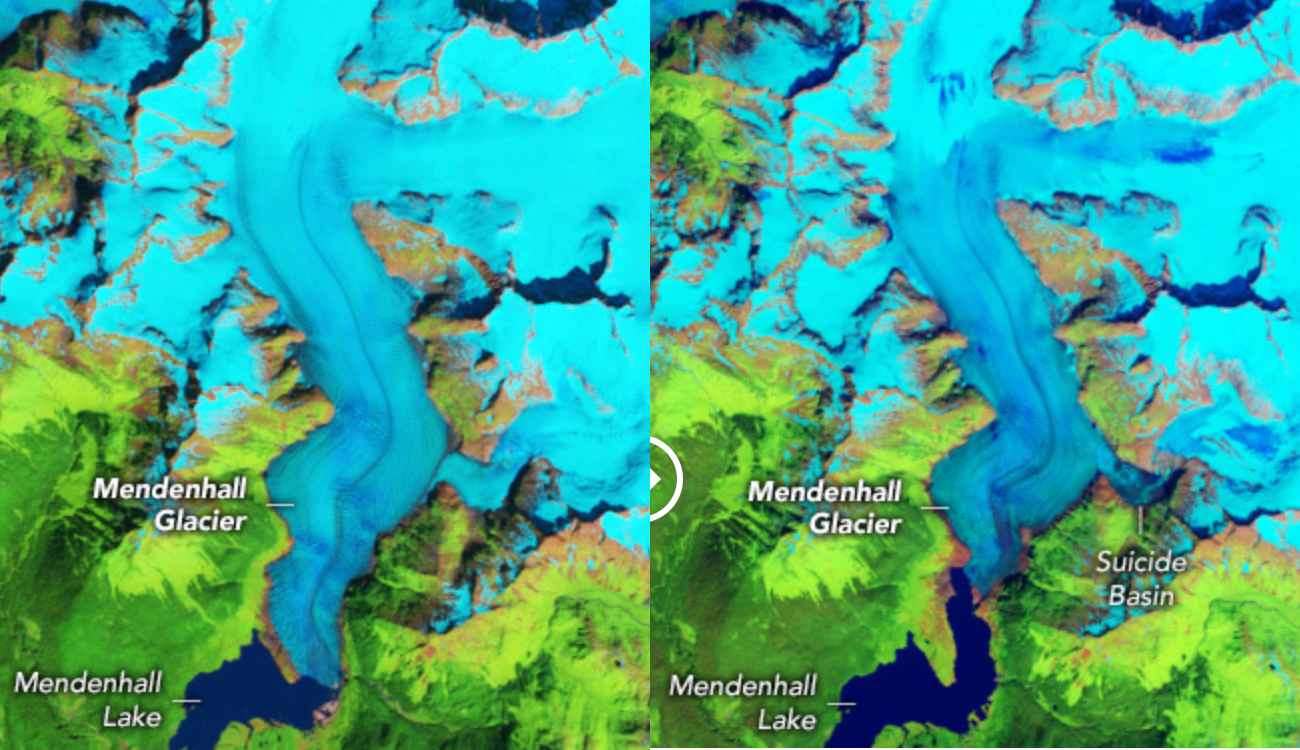
\includegraphics[width=.8\textwidth]{glacier.png}
	\caption{Volume Change of Mendenhall Glacier from August 17, 1984 to July 28, 2023}\label{fig:glacier}
\end{figure}

\subsection{Problem Restatement and Analysis}
\begin{itemize}
    \item \textbf{Problem1: }Develop a model for a sustainable tourism industry that should meet the maximization of revenue, the maximization of environmental quality, and the maximization of social satisfaction, and conduct a sensitivity analysis on it.
    \item \textbf{Problem2: }Demonstrate how the model can be adapted to another tourist destination affected by overtourism, by obtaining relevant information from another city and analyzing it with the model.
    \item \textbf{Problem3: }Develop a model to address the issue of visitor diversion, which is also a measure to increase revenue and reduce regional pressure.
    \item \textbf{An article: }Write a memo to the Juneau Convention and Visitors Bureau, outlining the forecast of the results, the impact of various measures, and suggestions on how to optimize the results.
\end{itemize}

\subsection{Our work}
To avoid complicated description , intuitively reflect our work process, the flow chart is show
as the following figure:
\begin{figure}[H]
	\centering
	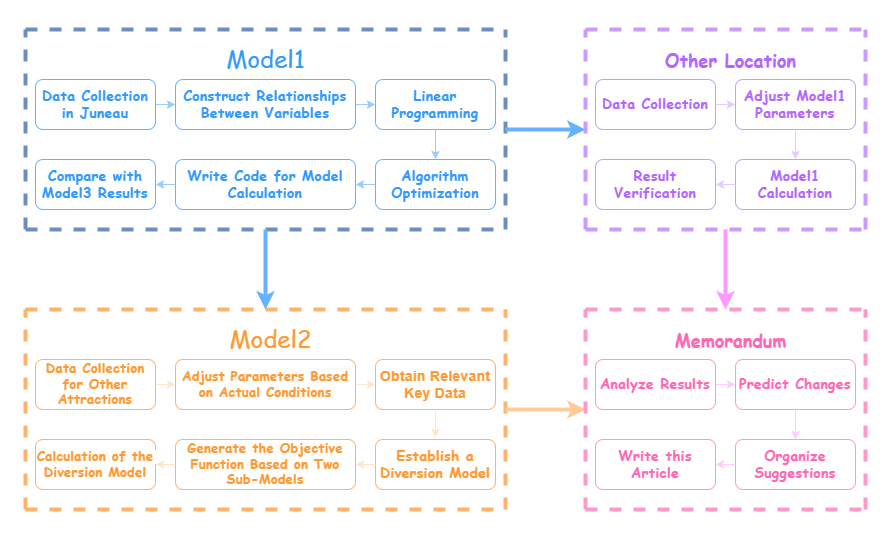
\includegraphics[width=\textwidth]{Process-map.png}
	\caption{Flowchart of Work}\label{fig:Process-map}
\end{figure}

\section{Preparation of the Models}
\subsection{Assumptions}
For Problem1:
\begin{itemize}
	\item Assuming that the positive impact of tourist consumption will drive indirect effects such as job creation, which can be uniformly measured by tourist consumption. To simplify the model, only the most important factor for the economic impact of tourism, namely tourist consumption, is considered, and indirect economic impacts such as job creation brought about by the development of tourism are not taken into account.
	%假设游客消费带来的正面影响会带动就业岗位等间接影响,总体可由游客消费统一衡量。为简化模型,只考虑对旅游业经济影响最重要的因素,即游客消费,不考虑旅游业发展带来的就业岗位等间接经济影响。
	\item It is assumed that changes in tax rates within a reasonable range will not have a significant impact on tourist consumption and the number of tourists. This is because increasing taxes does not significantly affect the growth in the number of tourists, and at the same time, it takes into account the combined effect of reduced willingness to consume and increased tourist consumption due to tax increases.
	%假设税收在一定合理范围内变动时不会对游客消费和游客人数产生剧烈影响。因为提高税收并没有对游客人数增长造成显著的影响,同时考虑到税收增长带来的消费意愿降低和游客消费提高的综合效应。
	\item To simplify the model, it is assumed that the per capita consumption of tourists is a constant. Based on the analysis of data from recent years, there has been no significant fluctuation in the per capita consumption of tourists, and it has not had a significant inhibitory effect on the number of tourists. It can be considered a constant when analyzing and optimizing for a shorter period of one year or several years.
	%为简化模型,假设游客人均消费为常数。由近几年的数据分析,游客人均消费并没有明显波动,对游客人数并没有明显的抑制作用,可认为在对一年内或近几年的较短周期的分析优化时是常量。
	\item Considering the infrastructure pressure and its associated implicit costs and environmental pollution, based on resident survey reports and actual conditions, the waste treatment system, which residents consider to be under the greatest pressure, and the water supply system, which is prone to stress, are chosen as representatives to measure implicit costs. It is assumed that the pressure conditions and trends of other aspects such as traffic pressure and energy supply are similar to these two, and their carrying capacities are used to measure them, ignoring their specific mathematical relationships in the model.
	%考虑基建压力与其所带来的隐性成本与环境污染,根据居民调查报告与实际情况,选择居民认为压力最大的废物处理系统,与容易出现压力的水供应系统作为隐性成本的代表进行衡量。假设其他如交通压力与能源供应等所受的压力情况与趋势与这两者相似,并由这两者的承载量衡量,在模型中忽略其具体的数学关系。
	\item It is assumed that expenditures can directly reflect in the carrying capacity and maximum carbon emissions, and enable their linear growth. To simplify the model and evaluation, considering the time-lag effect of investments on infrastructure and other aspects in the current year, it is simplified into a linear function, and the immediate benefits of expenditures are adjusted by regulating the coefficients in front of them.
	%假设支出能够直接反馈到承载量与最大碳排放量里面,并且使得其获得线性的增长。为简化模型与评测,综合考虑时间滞后效应下投入对当年的基建等的影响,将其简化为线性函数,并通过调节其前的系数调整支出的即时收益。
\end{itemize}

For Problem3:
\begin{itemize}
	\item It is assumed that the cost consumption of publicity and the number of people that can be diverted have a linear relationship to facilitate the quantitative calculation of publicity costs.
	%假设宣传的成本消耗与所能分流的人数为线性关系,以便于量化计算宣传成本。
\end{itemize}
% \subsection{数据准备}
% \begin{tabbing}
%     朱诺市近年的年游客数量 \= 朱诺市近年的月游客数量 \= 朱诺市税收分配情况 \kill
%     朱诺市近年的年游客数量 \> 朱诺市近年的月游客数量 \> 朱诺市税收分配情况 \\
%     朱诺市近年的各项税率 \> 朱诺市近年的游客人均消费 \> 朱诺市近年的游客调查报告 \\
%     朱诺市近年的居民调查报告 \> 朱诺市近年的饮用水年供应量 \> 朱诺市近年的日废物处理量 \\
%     美国居民日均用水量 \> 美国居民日均废物产生量 \> 九寨沟近年的年游客数量 \\
%     九寨沟近年的财政支出 \> 九寨沟近年的游客人均消费 \> 朱诺市观鲸项目项目报告 \\
%     朱诺市观鲸项目游客平均消费 \> 朱诺市观景项目近年年游客数量
% \end{tabbing}
\subsection{Notations}
The primary notations used in this paper are listed in the following Table.
% 三线表示例
\begin{longtable}{>{\centering\arraybackslash}m{4cm} >{\centering\arraybackslash}m{10cm}}
	\caption{Notations} \label{tb:notation} \\
	\toprule
	Symbol & Definition \\
	\midrule
	\endhead
	
	\midrule
	\multicolumn{2}{r}{\textit{Continued on next page}} \\
	\endfoot
	
	\bottomrule
	\endlastfoot
	
	\(R\) & Economic Development Index \\
	\(R_{e}\) & Total tourism income \\
	\(N_{t}\) & Number of tourists \\
	\(N_{tmax}\) & Maximum number of tourists allowed per year \\
	\(\tau_{t}\) & Tax rate \\
	\(P_{t}\) & Average spending per tourist \\
	\(E\) & Environmental Pollution Index \\
	\(CO_{2max}\) & Maximum allowed annual \(\text{CO}_{2}\) emissions \\
	\(CO_{2p}\) & Carbon emissions per person \\
	\(C_{waste}\) & The number of annual tourists that the city's waste treatment system can accommodate. \\
	\(C_{water}\) & The number of annual tourists that the city's drinking water supply system and water pollution treatment system can accommodate. \\
	\(S_{residents}\) & Residential satisfaction \\
	\(S\) & Social satisfaction \\
	\(P_{waste}\) & Cities' investment in waste management \\
	\(P_{water}\) & Cities' investment in water management \\
	\(P_{e}\) & Cities' investment in environment management \\
	\(Z\) & Representation of target equation\\
\end{longtable}

\section{Solution to Problem1}
\subsection{Establish a Sustainable Tourism Development Model}
\subsubsection{Identifying Relationships Between State Variables}
Considering the needs of sustainable tourism development, we evaluate the comprehensive benefits of Juneau's tourism industry from three perspectives: environment, economy, and society. Environmental pollution index $E$, economic index $R$, and social satisfaction index $S$ are set for the evaluation.
%考虑到可持续旅游发展的需要,我们从环境、经济与社会三个角度对朱诺市的旅游业综合收益进行评估。并设置环境污染指数E、经济指数R、与社会满意度指数S来进行评估。

Our objective function should be influenced by income, social satisfaction and environmental quality. We aim to maximize economic effects and social satisfaction while minimizing environmental pollution. Therefore, the economic index $R$ and social satisfaction index $S$ have positive effects on the objective function, while the environmental pollution index has a negative inhibitory effect on the objective function. Finally, we obtain:
%我们的目标函数应受收入,社会满意度和环境质量三者影响,我们希望经济效应最大化,社会满意度最大化以及环境污染最小化。故而,经济指数R与社会满意度指数S对目标函数起到正向的影响作用,而环境污染指数对目标函数有负向的抑制作用。最终我们得到:
\begin{equation}
	\text{Objective\ Function}:Z=R+S-E
\end{equation}

We mainly measure tourism income through the total expenditure of tourists during their travels. Total tourism revenue is mainly affected by per capita consumption and the total number of tourists. To simplify the model, we assume that per capita consumption will not fluctuate significantly in the short term and is a constant value. Therefore, the total tourism revenue should have a simple linear relationship with the number of tourists, so we can easily obtain Function 2.
%我们主要通过游客在旅游时的总消费来衡量旅游收入。旅游总收入主要受到人均消费金额与游客总人数的影响。为了简化模型,我们认为在短期内人均消费不会发生很大波动,是定值。故而旅游的总收入应当和旅客的人数成简单的线性关系,因此我们可以很简单的得到公式2
\begin{equation}
    R_{e}(N_{t},P_{t}) = P_{t}N_{t}
\end{equation}

It should be noted that since most tourism taxes, such as hotel taxes and alcohol taxes, are hidden taxes that are directly reflected in consumption, we consider that the tax revenue obtained by the government from the tourism industry is included in the calculated revenue, which is obtained by converting from the revenue according to the proportion of total tax revenue.
%需要注意的是,由于旅游的大部分税收,如酒店税与酒精税均是隐形税收,直接在消费中体现,故而我们认为政府从旅游业中获取的税收是包含在计算出的收入之中的,按照总税收的比例从收入中进行折算获得。

Meanwhile, in order to perform mathematical operations with environmental and social indices in the objective function for benefit evaluation, we normalized the per capita income to eliminate dimensional differences to obtain the objective function.
%同时,为了实现在目标函数中与环境和社会指数进行数学运算获得目标函数进行收益评估,我们对人均收入进行了归一化处理,消除量纲的差异以便于获得目标函数。
\begin{equation}
    R = R_{e}/R_{estandard}
\end{equation}
Where $R_{estandard}$ is the theoretical maximum value set for income. We believe that due to the need for environmental protection and other factors, the economy will not grow too much in the short term. Therefore, we select a constant slightly higher than the highest annual income in the most recent year as the maximum income to perform normalization and obtain the economic index.
%其中,$R_{estandard}$是设置的收入的理论最大值。我们认为,由于对环境保护等的需要,较短期内经济不会过大增长,选取略高于最近一年的年收入最高值的常数,作为收入最大值进行归一化处理获得经济指数。

In terms of environmental quality, we mainly consider the impact of three factors: carbon dioxide emissions, water consumption, and waste generation, all of which are closely related to the number of tourists.
%环境质量方面,我们主要考虑三个因素的影响:二氧化碳排放量,水的消耗量以及废物的产生量,而这三个因素都与游客人数密切相关。
For the carbon emission factor, we mainly consider the glacier melting problem in Juneau caused by excessive tourism. According to NASA data, the Mendenhall Glacier melted approximately 1.6 kilometers between 1984-2023 over 40 years, with an average melting rate of 40 meters per year, and its melting speed needs to be controlled. We can use the degree-day factor method to estimate the glacier melting rate:
%对于碳排放因素,我们主要考虑朱诺市由于过度旅游造成的冰川融化问题。根据NASA的数据,门登霍尔冰川在1984-2023年40年间融化了约16公里,平均每年融化40m,需要控制其融化的速度。我们可以使用度日因子法估计冰川的融化速度:
\begin{equation}
    M=DDF\times DDT
\end{equation}
Where DDF is the degree-day factor, which varies little and is close to constant, and DDT is the positive temperature sum, which is directly affected by temperature. To control the rate of glacier melting, the key is to control temperature rise, and carbon emissions are the main factor affecting temperature rise. According to the \textit{Paris Agreement}, the average annual temperature rise between 1850-2100 should be controlled between 1.5-2.0 degrees, and we use 1.5 degrees as the maximum temperature rise to calculate the maximum carbon emissions.
%其中,DDF是度日因子,变化小接近常量,而DDT是正积温,受到温度的直接影响。想要控制冰川融化的速度,关键在于控制温度的升高,而碳排放是影响温度升高的主要因素。根据《巴黎协定》的规定,1850-2100年间年平均气温升高尽量控制在1.5度-2.0度,我们以1.5度为温度升高的最大限度计算最大碳排放量。
\begin{equation}
    \Delta T=\lambda\times \ln(CO_{2}/CO_{2pre-industrial})
\end{equation}
According to this formula, we calculate the global average increase in carbon dioxide concentration, multiply it by atmospheric mass to obtain the total global carbon dioxide emissions over 250 years, and estimate Juneau's average annual emissions through its population proportion. Tourism is Juneau's largest industry, accounting for 60 percent of total emissions. Meanwhile, we calculate the maximum carbon emissions by adding the forest wetland area and average carbon absorption of Juneau.
%根据该公式计算出全球平均二氧化碳浓度增量,乘上大气质量得到全球250年间的二氧化碳排放总量,通过朱诺市的人口占比,估算出朱诺市的年平均排放量。旅游业是朱诺市占比最大的产业,按照总量的百分之60计算排放总量。同时我们根据朱诺市的森林湿地面积与平均碳吸收量,将两者相加得到最大碳排放量。
As for tourists' per capita carbon footprint, we considered that tourists mainly travel by cruise ships, which have relatively high carbon emissions, and estimated per capita carbon emissions by combining the average carbon emissions of cruise travel and tourists' onshore activities.
%而对于游客的人均碳足迹,我们考虑到游客主要以邮轮方式出行,有较高的碳排放量,结合邮轮出行平均碳排放量和游客岸上行动的平均碳排放量对人均碳排放量进行了估计。
Through Juneau's processing capacity for the latter two factors and the per capita consumption/generation of tourists and residents, we can calculate the number of tourists that Juneau's water supply system and waste treatment system can accommodate annually, $C_{waste}$ and $C_{water}$. We normalize the actual number of people compared to the carrying capacity to measure the pressure on the infrastructure system. Finally, combining the importance factors of each factor, we obtained Function 3:
%通过朱诺市对后两个因素的处理能力和游客与居民的人均消耗/产生量,可以计算出朱诺市供水系统和废物处理系统可以每年承载的游客数$C_{waste}$, $C_{water}$,我们将实际的人数和承载人数相比进行归一化处理来衡量基建体系压力。最后结合各因子的重要性因素得到了公式3:
\begin{equation}
	E=k_{1}\frac{CO_{2p}N_{t}}{CO_{2max}}+k_{2}\frac{N_{t}}{C_{waste}}+k_{3}\frac{N_{t}}{C_{water}}
\end{equation}
Specifically, we believe that Juneau currently faces a relatively serious glacier melting problem and needs to control carbon emissions. Additionally, its waste treatment system has a smaller capacity compared to its water supply system, and population growth puts greater pressure on it. Therefore, we consider $k_1>k_2>k_3$.
%具体的,我们认为朱诺市目前面临较为严重的冰川融化问题,需要控制碳排放量,同时,其废物处理系统的承载量相比供水系统更小,人数的增长对其的压力更大,故而我们认为k1>k2>k3。

Regarding social satisfaction, since tourist satisfaction has shown no significant changes in statistical data over a long time span, with overall satisfaction remaining around 99\%, we believe that tourist satisfaction will not change significantly when factors like taxation are reasonable. Therefore, we mainly consider resident satisfaction.
We primarily collected social satisfaction survey results from Juneau for five years: 1998, 2002, 2006, 2022, and 2023\cite{4}. After excluding invalid evaluations marked as "no impact" and "don't know," the remaining evaluations were categorized into five levels according to the Likert scale. We converted the data scoring to a 100-point scale. Additionally, we looked up the tourist numbers for these five years\cite{5} and performed data fitting with social satisfaction, obtaining the following results:
%社会满意度方面,由于游客满意度在较长时间跨度的统计数据中均无明显变化,总体满意度停留在百分之99左右,我们认为游客满意度在税收等合理的情况下不会发生明显变化,故而主要考虑居民满意度。
%我们主要收集了朱诺市1998,2002,2006,2022,2023五年的社会满意度调查结果\cite{4},摒除其无影响和不知道的无效评价,剩下的评价依据李斯特量表分成了五级,我们按照100分制对数据的评分进行了扩大处理。同时我们查找了这五年的游客人数\cite{5}来和社会满意度进行了数据拟合并得到了如下结果:
\begin{figure}[H]
	\centering
	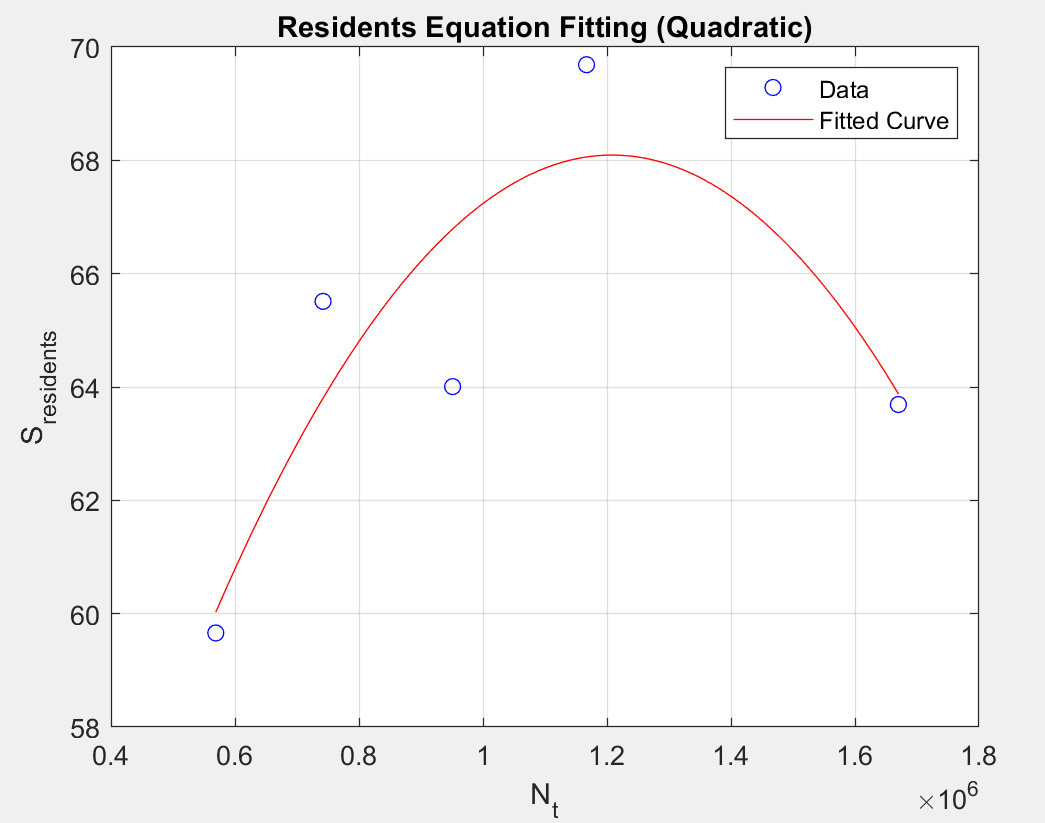
\includegraphics[width=.8\textwidth]{satisfaction.png}
	\caption{Nonlinear Fitting between $N_t$ and $S_{residents}$}\label{fig:satisfaction}
\end{figure}
Where $a_1 = -1.9753 \mathrm{e}{-11}$, $a_2 = 4.772\mathrm{e}{-5}$, $b = 39.2660$, $R^2 = 0.7423$. Finally, to eliminate the impact of dimensionality, we divided the satisfaction score by the maximum satisfaction value of 100 points. The resulting Function 4 is as follows:
%其中,$a_1 = -1.9753 \mathrm{e}{-11}$, $a_2 = 4.772\mathrm{e}{-5}$, $b = 39.2660$, $R^2 = 0.7423$。最后,为了消除量纲带来的影响,我们给满意度除以了满意度的最大值100分。得到的公式4如下:
\begin{equation}
	\begin{cases}
		S_{residents}=a_{1}N_{t}^2+a_{2}N_{t} + b_{1} \\
		S=S_{residents}/100
	\end{cases}
\end{equation}

In terms of additional investment, we considered the feedback effect of the government's tax allocation plan on the system. The government can invest in water supply systems, waste treatment systems, and environmental protection, such as infrastructure construction or increasing afforestation efforts, to improve the maximum carrying capacity of infrastructure and maximum carbon emissions, thereby obtaining higher returns. We believe that the government can adjust the proportion of investment in actual government allocation to maximize returns. The resulting Function 5 is as follows:
%额外投入方面,我们考虑到了政府对于额外税收的分配计划对系统的反馈作用,政府可以向供水系统、废物处理系统以及环境保护方面进行投入,如进行基建建设或者增强植树造林等,以提高基建的最大承载量和最大的碳排放量,进而获取更高的收益。我们认为政府可以调整投入在政府实际分配中的比值,以获取最大的收益。得到公式5如下:
\begin{equation}
	\begin{cases}
		P_{waste} = k_5\tau_tR_e\\
		P_{water} = k_6\tau_tR_e\\
		P_{e}=k_7\tau_{t}R_e \\
		k_5+k_6+k_7 \leqslant 0.4
	\end{cases}
\end{equation}
To simplify the model, we assume that investment can directly generate returns, and expenditures directly increase infrastructure carrying capacity or maximum carbon emissions at a certain ratio, in order to facilitate model decision-making.
%为了简化模型,我们认为投入能够直接带来回报,并且支出以一定比例直接增加基建承载量或者最大碳排放量,以便于模型做出决策。
\begin{equation}
	\begin{cases}
		C_{waste}+=\alpha_1P_{waste} \\
		C_{water}+=\alpha_2P_{water} \\
		CO_{2max}+=\alpha_3P_e \\
	\end{cases}
	\end{equation}

\subsubsection{Find the constraints}
In terms of economics, to limit the tax rate value and ensure the accuracy of assumptions, we set a restriction that the overall tax rate should be less than or equal to 8\%. Therefore, we have Formula 7:
%在经济方面,为了限制税率的值以保证假设准确,我们设置了一个限制,认为总体税率应小于等于8\%。因此有公式7:
\begin{equation}
	\text{Financial}:\tau_{t}\leqslant 8\% \\
\end{equation}

Regarding tourist numbers, based on Juneau's policy\cite{6}, we derived the daily tourist number limit. Function 8 is as follows:
%游客人数方面,我们依据朱诺市的政策\cite{6}得出了每天的游客的人数限制。公式8如下:
\begin{equation}
	\text{Touristic}:
		0\leqslant N_{t}\leqslant N_{tmax}\\
\end{equation}

Regarding environmental aspects, first, we set a limit on the maximum carbon dioxide emissions. For the maximum carrying capacity of water resources and waste treatment, we considered that seasonal fluctuations in tourist numbers would lead to increased infrastructure pressure during peak seasons. Based on the data, we obtained the ratio of maximum daily tourist numbers during peak season to total annual tourist numbers. Taking into account the elasticity of infrastructure capacity within a year, we set 1.2 times the daily average carrying capacity as an upper limit to restrict the maximum daily number of tourists. Function 9 is as follows:
%环境方面,首先,我们限定了二氧化碳的最大排放量,而在水资源最大承载量和废物处理最大承载量上面,我们考虑到游客人数的季节性波动会导致旺季基建压力的上升,根据数据获得旺季每天最多游客人数占全年总游客人数的比例,考虑到基建能力一年内的的承载弹性,升大设置1.2倍日平均承载量作为上限来限制最大的日游客人数。公式9如下:
\begin{equation}
	\text{Environmental}:
	\begin{cases}
		N_{t}\cdot CO_{2p}\leqslant CO_{2max} \\
		0.012N_t\leqslant \frac{1.2}{365}C_{waste} \\
		0.012N_t\leqslant \frac{1.2}{365}C_{water}
	\end{cases}
\end{equation}

Regarding social satisfaction, after appropriate quantification, we set 60 as the passing threshold. Therefore, Function 10 is as follows:
%社会满意度方面,经过合适的量化后,我们将60作为及格线。故公式10如下:
\begin{equation}
	\text{Social}:\ S_{residents} \geqslant 60
\end{equation}	

\subsubsection{Multi-start Optimization Algorithm}
Since our model has five decision variables, namely \(N_t\), \(\tau_t\), \(k_5\), \(k_6\) and \(k_7\), which interact with each other and have varying degree of influence on the objective function. In order to achieve relatively optimal conditions for each decision variable locally and at the same time strive for the global objective to be optimal, such as maximizing tourism revenue, minimizing environmental impact, and maximizing resident satisfaction, etc., we use a multi-start optimization strategy to optimize the various influencing factors of the objective function. The pseudocode is as follows:
\begin{breakablealgorithm}
	\caption{Multi-start Optimization Algorithm}
	\begin{algorithmic}[1]
		\STATE \textbf{Input:} $n\_starts$,\ $Nmax$
		\STATE \textbf{Output:} $best\_result$
		\vspace{0.2cm}
		\STATE /* Initialize variables */
		\STATE $best\_result\leftarrow null$
		\STATE $best\_objective\leftarrow \infty$
		\STATE /* Generate starting points for each parameter */
		\STATE $Nt\_starts\leftarrow linspace(100000,\,0.8\times Nmax,\,n\_starts)$
		\STATE $\tau\_starts\leftarrow linspace(0.02,\,0.07,\,n\_starts)$
		\STATE $k\_starts\leftarrow linspace(0.05,\,0.15,\,n\_starts)$
		\vspace{0.2cm}
		\STATE \textbf{Define optimization bounds}
		\vspace{0.2cm}
		\STATE /* Perform optimization from multiple starting points */
		\FOR{$i\leftarrow 0$ \TO $n\_starts-1$}
		\STATE /* Construct initial point */
		\STATE $x0\leftarrow [Nt\_starts[i],\ \tau\_starts[i],\ k\_starts[i],\ k\_starts[i]]$
		\STATE /* Minimize objective function */
		\STATE $result\leftarrow \textbf{minimize\_function}$
		\STATE /* Update best result if better solution found */
		\IF{$result.success$ \AND $result.objective\ <\ best\_objective$}
		\STATE $best\_objective\leftarrow result.objective$
		\STATE $best\_result\leftarrow deepcopy(result)$
		\ENDIF
		\ENDFOR
		\vspace{0.2cm}
		\RETURN $best\_result$
	\end{algorithmic}
\end{breakablealgorithm}

\textbf{The solution and output of the model:} The model maximizes economic, environmental, and social benefits through multi-start optimization of five decision variables. In the initialization phase, the algorithm first sets up an empty optimal solution container and an infinite initial optimal objective value as the benchmark. Then, the algorithm generates multiple sets of different starting points within reasonable value ranges to ensure that the algorithm can explore a larger solution space. During the optimization loop phase, the algorithm performs a complete optimization attempt for each set of starting points. Each attempt uses the \textbf{Sequential Least Squares Quadratic Programming} (SLSQP) method to find the solution that optimizes the objective function, considering all constraints, such as visitor number limits, tax rate range, investment ratio restrictions, etc.). If an optimization attempt is successful and the resulting objective function value is better than the currently recorded optimal value, the optimal solution and objective value are updated. This process repeats until all starting points have been tested, and the globally optimal result is retained.

\subsubsection{Calculation Results}
Regarding total tourism revenue, based on historical data, we assign the value x to the average tourist expenditure. Through our calculations, we can determine that the annual number of tourists should be 1,431,579 people, with $P_e$ being \$4272,000,000,000. Looking at historical data, this figure appears relatively reasonable.
%旅游总收入上,根据以往的数据,我们给旅客平均消费值赋值为x。经过我们的计算可以得到游客每年人数应为1431579人,$P_e$为272000000000美元,结合以往的数据来看,这个数据是相对合理的。

Regarding resident satisfaction, after inputting the number of tourists into the fitting equation, we obtain a resident satisfaction score of 67.18, which falls within our expected range.
%居民满意度上,将旅客人数带进拟合方程后可以得到居民满意度为67.18,符合我们的预期范围。

Regarding environmental quality, through calculations, we obtained $k_5 = 0.179$, $k_6 = 0.113$, $k_7 = 0.108$. After substituting the number of tourists, $\text{CO}_{2max}$, $C_{waste}$, $C_{water}$, and $N_t$ into the equation, we got a result of 0.4876, which falls within our expected range.
%环境质量上,通过计算得出$k5 = 0.179$, $k6 = 0.113$, $k7 = 0.108$,将旅游人数和$CO_{2max}$, $C_{waste}$,$C_{water}$, $N_t$带入方程后得出结果为0.4876,符合我们的预期范围。

\subsection{Sensitivity Analysis}
Since we have used a multi-start optimization strategy, we use \textbf{Sobol Analysis} to simultaneously analyze the local sensitivity and global sensitivity of the input variables $N_t$, $\tau_t$, $k_5$, $k_6$ and $k_7$. The pseudocode is as follows:
\begin{breakablealgorithm}
	\caption{Sensitivity Analysis}
	\begin{algorithmic}[1]
		\STATE \textbf{Input:} $n\_samples$
		\STATE \textbf{Output:} $Si$ (result of Sobol Analysis)
		\vspace{0.2cm}
		\STATE /* Define problem structure */
		\STATE \textbf{Initialize problem dictionary:}
		\STATE $\quad$number of variables, variable names, variable bounds
		\STATE /* Generate samples */
		\STATE $param\_values = saltelli.sample(problem,\ n\_samples)$
		\STATE /* Evaluate model for all samples */
		\STATE Initialize empty array $Y$
		\FOR {each parameter set $X$ in $param\_values$}
		\STATE Calculate objective function value for $X$
		\STATE Add result to array $Y$
		\ENDFOR
		\STATE /* Normalize results */
		\STATE $Y = (Y - minimum\ of\ Y) / (maximum\ of\ Y - minimum\ of\ Y)$
		\STATE /* Perform Sobol Analysis */
		\STATE $Si=sobol.analyze(problem,\ Y)$
		\vspace{0.2cm}
		\STATE \textbf{Print results}
		\STATE \textbf{Visualize results}
		\vspace{0.2cm}
		\RETURN $Si$
	\end{algorithmic}
\end{breakablealgorithm}

The results are shown in the figure below:
\begin{figure}[H]
	\centering
	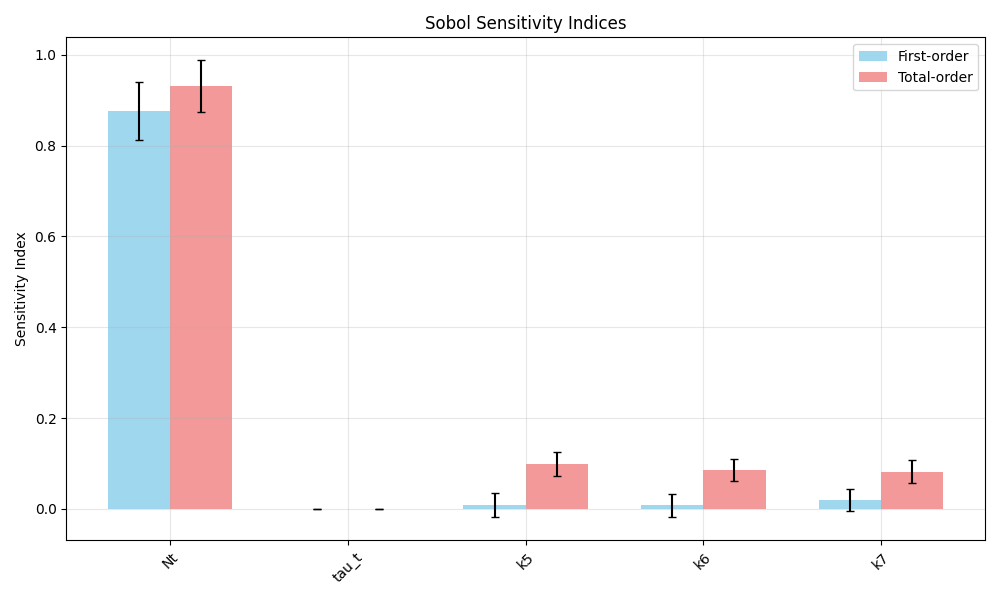
\includegraphics[width=.8\textwidth]{sensitive.png}
	\caption{Sensitivity Analysis}\label{fig:sensitivity}
\end{figure}

From the figure, it is clear that the number of tourists is the most critical variable, with its local and global sensitivities reaching $0.877$ and $0.932$, respectively, far greater than the other input variables. This also aligns with the objective fact that, as a tourist city, Juneau's income is heavily influenced by the number of tourists.

\subsection{Model Validation}

In Section 3.1, we used a multi-starting point hybrid optimization strategy to calculate our established sustainable tourism development model, and conducted sensitivity analysis in Section 3.2. Although our calculation results were relatively consistent with reality, we still raised some doubts about their accuracy. Therefore, we employed a multi-objective optimization strategy to recalculate the optimal conditions for the above model to verify the correctness of the multi-starting point hybrid optimization strategy in Section 3.1. Our optimization objectives remained maximizing income, minimizing environmental impact, and maximizing social satisfaction. In the new multi-objective optimization strategy, we used the DEAP (Distributed Evolutionary Algorithms in Python) framework to implement NSGA-II (Non-dominated Sorting Genetic Algorithm II). We then used Pareto optimization to obtain a series of optimal conditions under this model, and based on requirements and actual situations, selected the final result range between 1,300,000 and 1,450,000. This result both met our expectations and corroborated the results from the multi-starting point hybrid optimization strategy in Section 3.1. Additionally, we also performed Sobol sensitivity analysis on the multi-objective optimization strategy algorithm, obtaining results that were very similar to those in Section 3.2, which further proved the correctness of both the multi-objective optimization strategy algorithm in Section 3.3 and the multi-starting point hybrid optimization strategy algorithm in Section 3.1. The figure shows the execution results of the multi-objective optimization strategy algorithm.
%在3.1中,我们使用多起点的混合优化策略,计算了我们建立的可持续旅游发展模型,并在3.2中对其进行了敏感度分析。虽然我们的计算结果比较符合实际,但我们仍对其正确性提出了一些质疑。因此,我们又使用了多目标优化策略再次计算了以上模型的最优情况,以验证3.1中多起点的混合优化策略的正确性。我们的优化目标依然是收入最大化、环境影响最小化和社会满意度最大化。在新的多目标优化策略中,我们使用了DEAP(Distributed Evolutionary Algorithms in Python)框架来实现NSGA-II(非支配排序遗传算法II)。然后我们使用帕累托优化,得到该模型下的一系列最优情况,然后根据需求和实际情况,选取最终的结果范围在1300000到1450000之间。这一结果既符合我们的预期,也于3.1中的多起点混合优化策略的结果相互印证。此外,我们同样对多目标优化策略的算法进行了Sobol敏感度分析,得到的结果与3.2中的结果相差无几,这也进一步证明了3.3中的多目标优化策略算法的正确性,以及3.1中多起点的混合优化策略算法的正确性。如图是多目标优化策略算法的执行结果。

\begin{figure}[htbp]
\centering
\begin{subfigure}[b]{.4\textwidth}
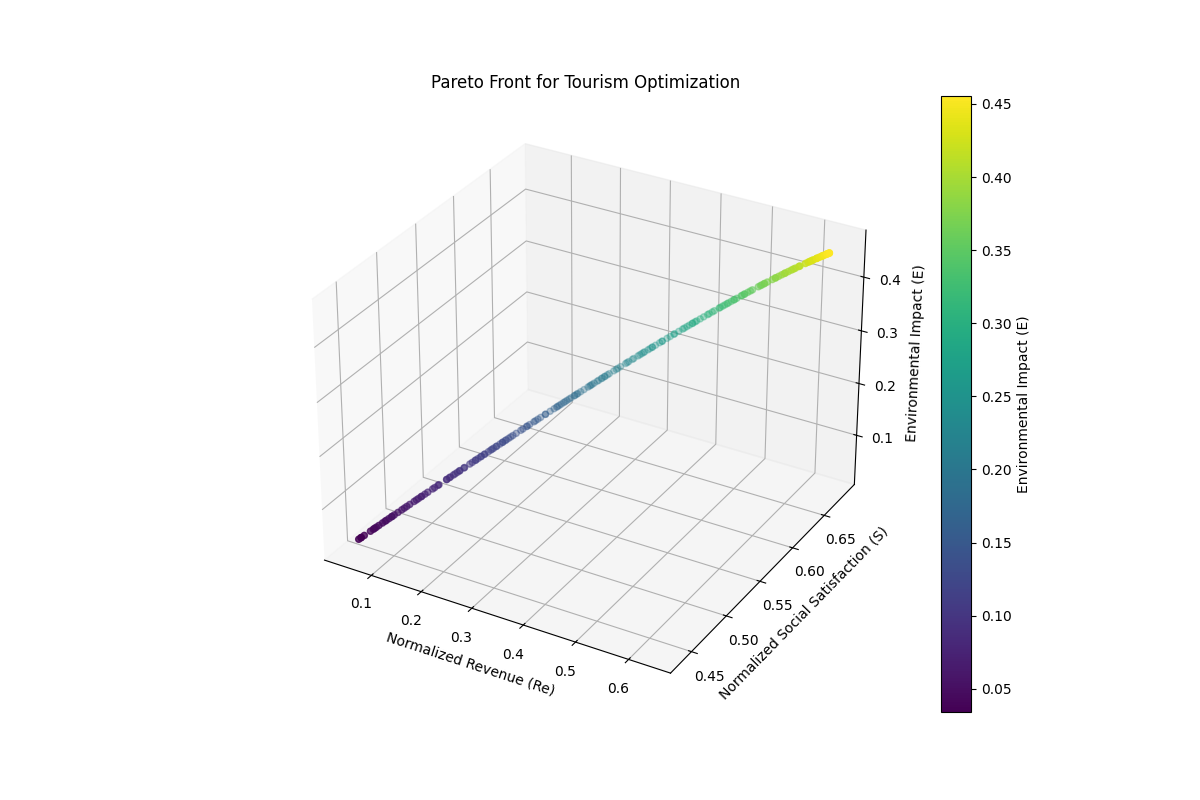
\includegraphics[width=\textwidth]{pareto1.png}
\caption{Pareto Front 1}\label{subfig:left1}
\end{subfigure}
\begin{subfigure}[b]{.4\textwidth}
	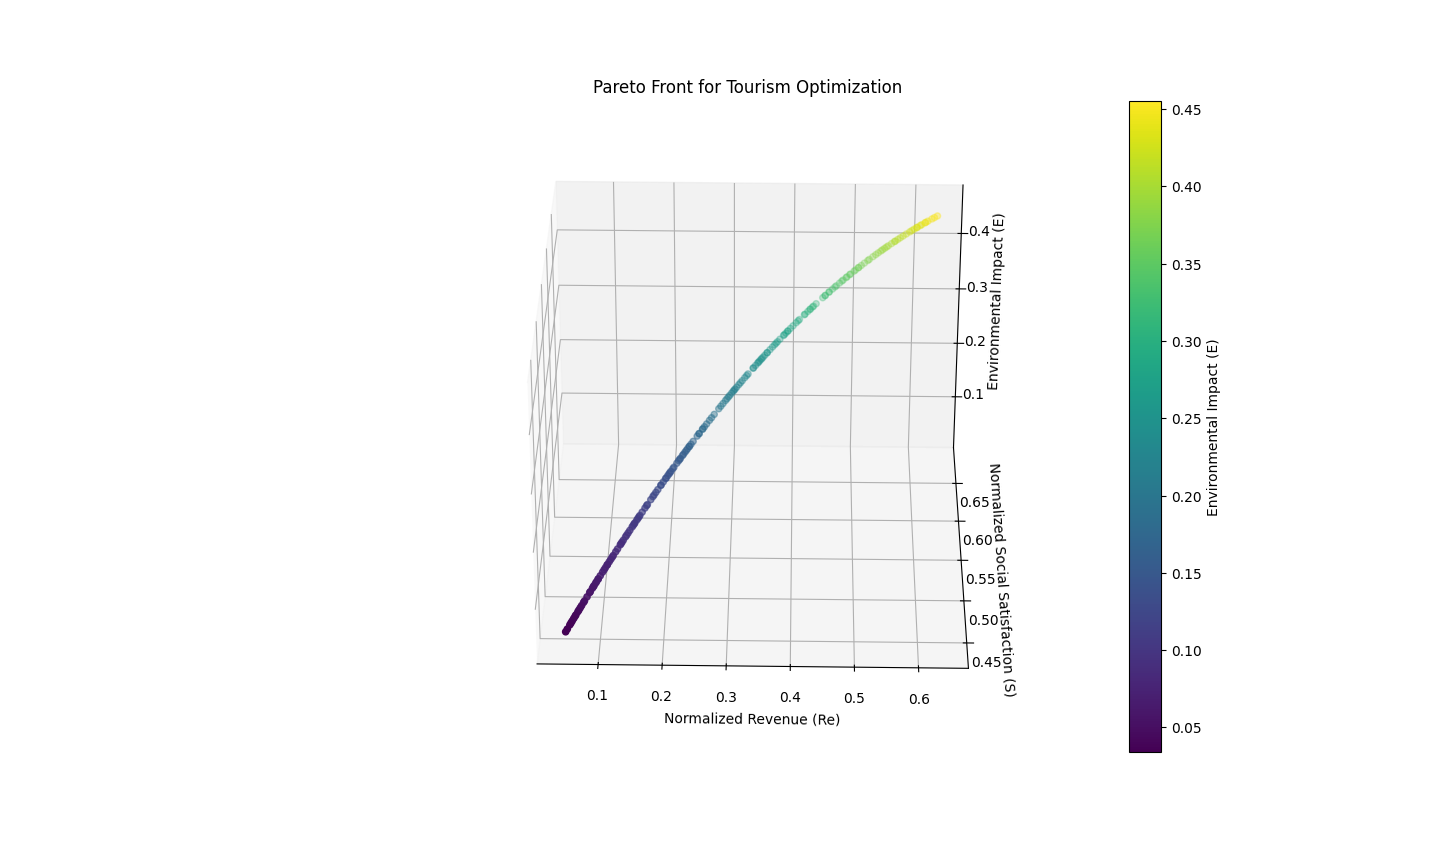
\includegraphics[width=\textwidth]{pareto2.png}
	\caption{Pareto Front 2}\label{subfig:right1}
\end{subfigure}
\end{figure}

\begin{figure}[htbp]
	\centering
	\begin{subfigure}[b]{.4\textwidth}
		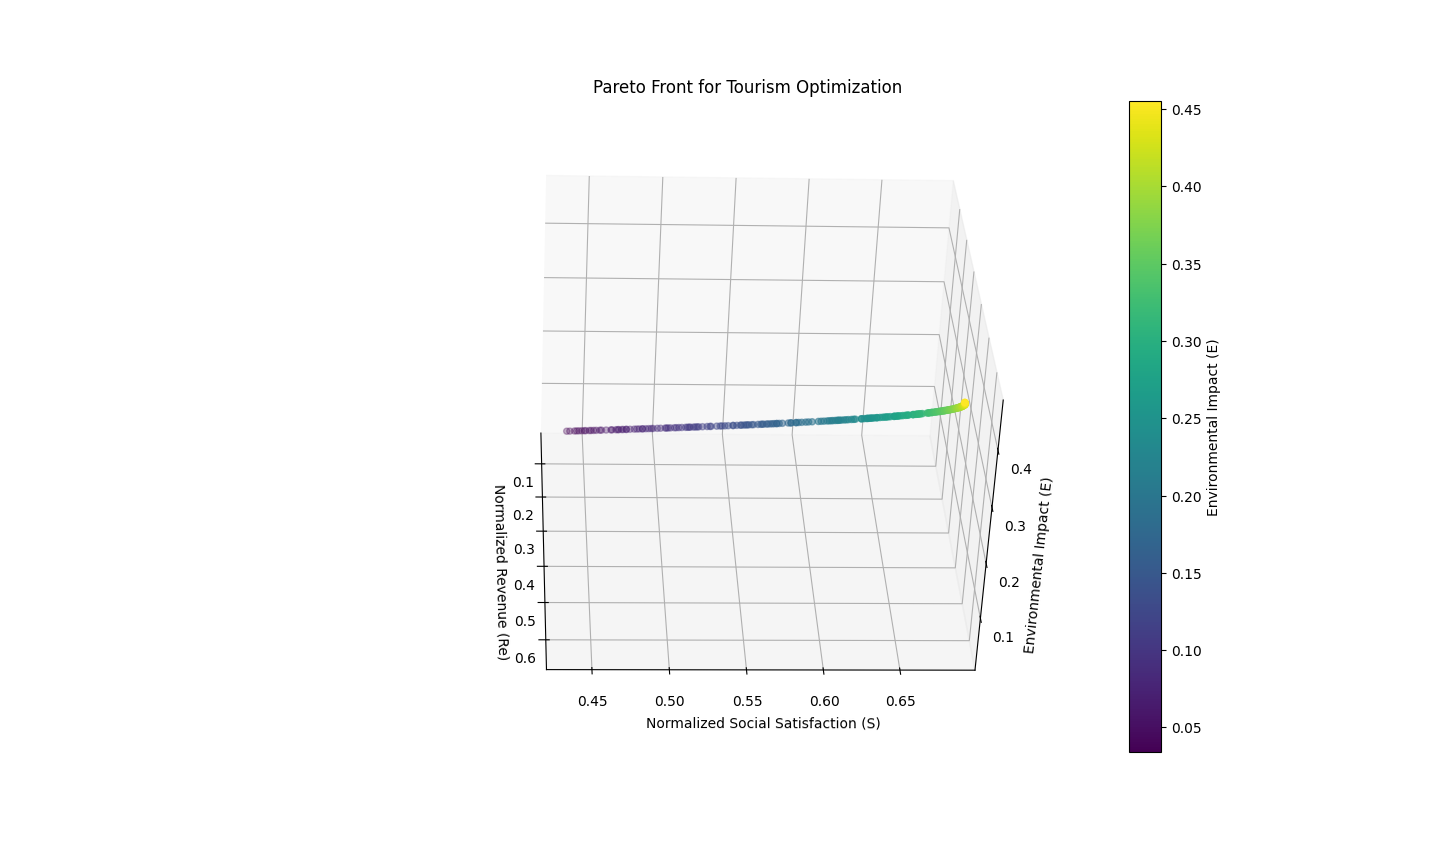
\includegraphics[width=\textwidth]{pareto3.png}
		\caption{Pareto Front 3}\label{subfig:left2}
	\end{subfigure}
	\begin{subfigure}[b]{.4\textwidth}
		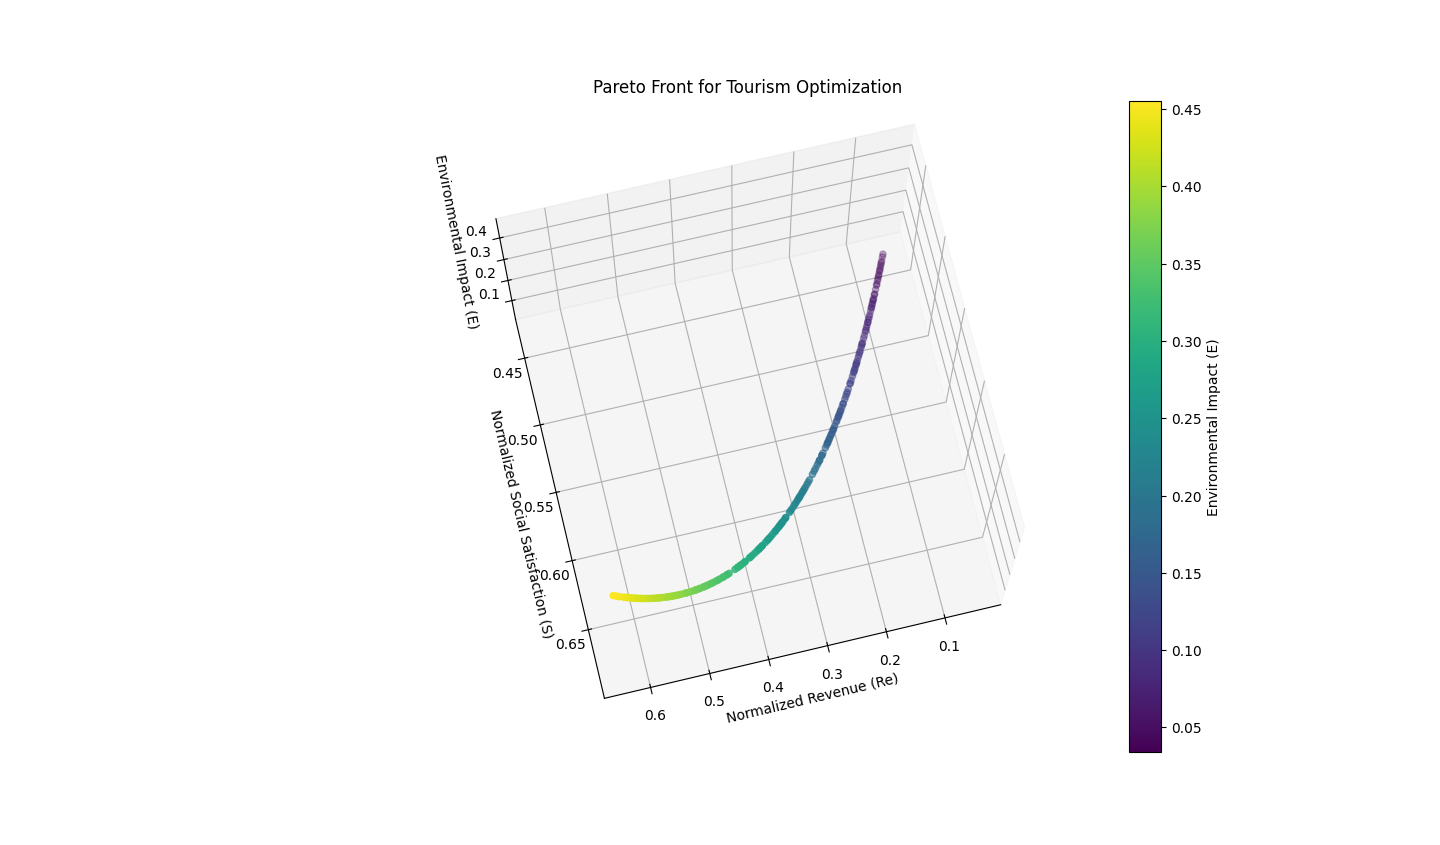
\includegraphics[width=\textwidth]{pareto4.png}
		\caption{Pareto Front 4}\label{subfig:right2}
	\end{subfigure}
\end{figure}

\section{Solution to Problem2}
为了展示模型是如何适应另一个受过度旅游影响的,我们经过数据的查找和收集决定选择位于中国四川省的九寨沟风景区来进行分析。
\subsection{数据收集}
因为每个地方的基础设施压力,人均消费等都大不相同,我们需要经过数据调研修改相应的参数后才能使用当前的模型进行预测。

通过对官网数据的收集\cite{8},我们可以得出九寨沟县每年的收入和九寨沟风景区之间的关系。但是由于官方网站缺乏相应的满意度调查等信息,我们根据社会上的普遍评价对这些值进行了简单的估计,通过修改相应的限制条件,如水资源的人均消耗量,废物的人均产生量,水资源和废物处理的承载能力,游客人均消费水平,我们可以将模型适用于九寨沟的情况。
\begin{figure}[H]
	\centering
	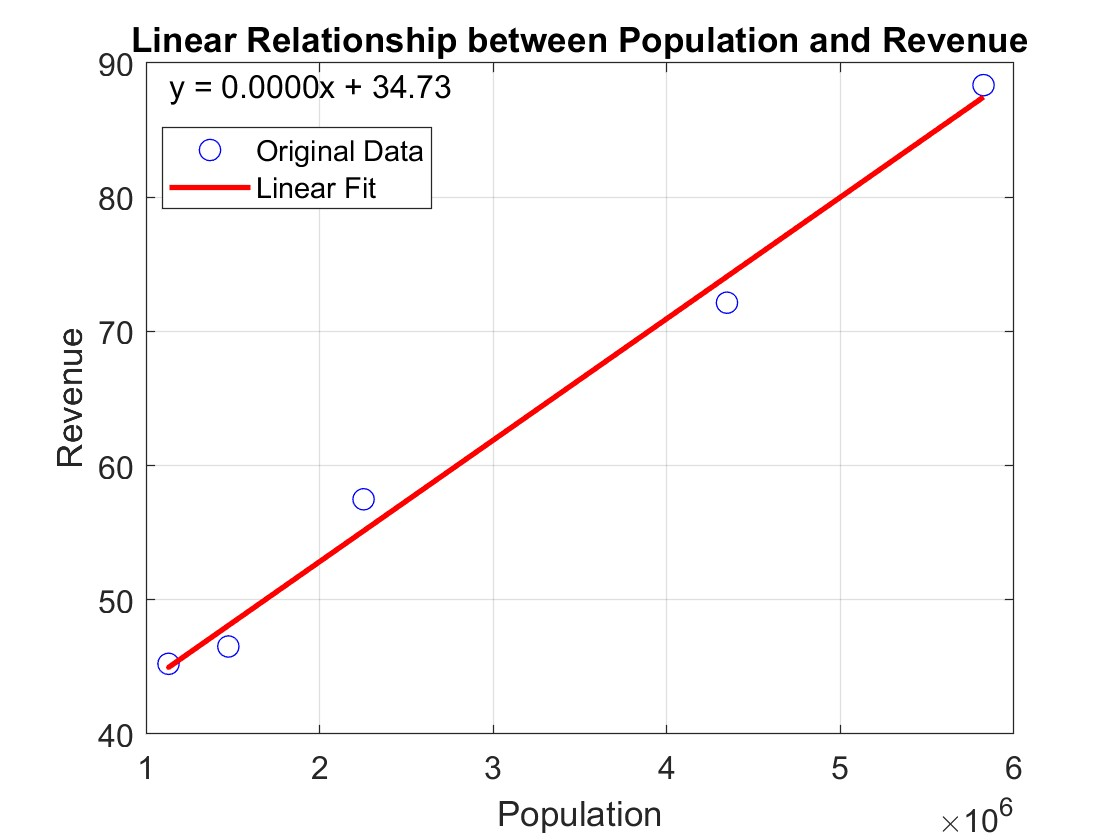
\includegraphics[width=.8\textwidth]{JiuZhaiGou.jpg}
	\caption{The Relationship between Tourism Revenue and Number of Visitors in Jiuzhaigou Scenic Area}\label{fig:JiuZhaiGou}
\end{figure}
\subsection{结果展示}
根据我们模型跑出来的最佳结果显示,$N_t$为3747368,$P_e$为2248421052.70元,$S_{residents}$为65.10,$k5$为0.169,$k6$为0.123,$k7$为0.108。这些结果与往年数据相比较具有合理性。

\section{Solution to Problem3}
\subsection{生成不同景点的可持续发展模型}
为了进行不同景点之间分流,我们需要获取各个景点的可持续发展模型以确定发展策略,便于获取在某个实际游客数量下的综合收益。因此,我们需要获得具体每个景点的相关数据。因为不同景点的环境条件、人均消费、基建承载量等不同,游客人数导致的基建压力和社会满意度也大不相同,所以我们需要修改模型一的参数以来适应不同景点的实际情况。

我们主要考虑对朱诺市的两个人们景点门登霍尔冰川和赏鲸雨林进行分析。在模型一的基础上,我们搜集了赏鲸的相关数据,包括赏鲸项目的年游客人数、平均游客消费等,并对相关的参数进行了调整,由于参与赏鲸景点的游客同样主要在朱诺市附近活动,我们考虑赏鲸景点的最大承载量等与门登霍尔冰川的近似,同时,由于赏鲸项目并未面临很严重的环境问题,我们上调了最大碳排放量,以及环境投资的回报系数,以更好地模拟实际的情况。
我们对两个模型分别进行了单独的优化计算,获取到了最优游客人数,最优税收以及最优的支出分配策略,接着,我们构建了分流模型以优化实际的分流人数。
\subsection{建立分流模型}
假设模型中有$n$个子模型,代表了具体的$n$个景点。
每个模型中的实际人数为$N_{ti}$,,最优人数为$N_{ei}$。对于实际人数大于最优人数的景点$n_i$,我们希望将超出最优人数的部分分流去实际人数较少的景点$n_j$,则
$C_{i-j} = C_{pi-j}*\Delta N_{i-j}$,代表此次分流的总成本等于将一个人从$n_i$分流到$n_j$的宣传成本乘以分流走的人数,则宣传成本总共为$C = \sum_{i,j} C_{i-j}$,
故决策变量为:
\begin{equation}
    \Delta N_{i,j} (1 \leq i,j \leq n)
\end{equation}
目标函数为:
\begin{equation}
	Z = \sum_{i=1}^{n} Z_i(N_{ti}) - \frac{C}{C_{std}}
\end{equation}
其中,$C_{std}$是估计的最大宣传成本,用于进行归一化去除宣传支出的量纲。
\subsection{计算结果}
这里以朱诺市两个景点门登霍尔冰川和赏鲸景点为例来具体展示分流模型的结果。
我们希望将游客从门登霍尔冰川分流至赏鲸景点以减少冰川面临的环境压力,我们首先对两个子模型进行了分别的优化,计算出了最佳人数、税率与支出分配比例,并将其作为输入调整分流模型。紧接着我们估计了分流每人的大致宣传成本,输入到分流模型中完成了模型的构建。
具体的,我们采用模拟退火算法进行求解。通过设定一个初始温度,控制步长大小,模拟固体退温的过程,以求解模型的全局最优解。
经过计算,我们得出分流人数在329888人左右最佳,分流比例达到在百分之二十左右。参考我们模型的结果,朱诺政府可以考虑采取更好的宣传策略,以获取更好的总体收益。


% 以下为信件/备忘录部分,不需要可自行去掉
% 如有需要可将整个 letter 环境移动到文章开头或中间
% 请在第二个花括号内填写标题,如「信件」(Letter)或「备忘录」(Memorandum)
\begin{letter}{Memorandum}
\begin{flushleft}  % 左对齐环境,无首行缩进
\textbf{To:} 朱诺市政府\\
\textbf{From:} Team 2510625\\
\textbf{Date:} January 27th, 2025\\
\textbf{Subject:} 关于政府在旅游业上的一些建议
\end{flushleft}

随着旅游市场的不断发展,朱诺市作为阿拉斯加的首府,拥有丰富的自然景观和独特的文化魅力,吸引了大量游客前来观光旅游。为了更好地了解旅游市场的发展趋势,评估各种措施对旅游市场的影响,并提出优化建议,我们进行了深入的市场调研和数据分析。

首先是关于旅游市场的预测,根据我们的市场调研和数据分析,预计未来几年朱诺市的旅游市场将呈现以下趋势:
\textbf{游客数量增长:}随着全球经济的复苏和人们生活水平的提高,预计未来几年朱诺市的游客数量将呈现稳步增长的趋势。特别是来自亚洲和欧洲的游客数量将有较大幅度的增加。
\textbf{旅游季节变化:}虽然夏季仍然是朱诺市的旅游旺季,但随着冬季旅游项目的不断丰富,如狗拉雪橇、冰钓等,冬季旅游市场也将逐渐升温。

二是各种措施的影响,为了促进朱诺市旅游市场的发展,我们分析了一系列措施,这些措施对旅游市场产生了以下影响:
\textbf{适量提高税率:}适量提高税率短时间不会对旅游人数产生较大的影响,而税率的提高可以增加旅游业带来的收入,额外收入增加后可以对基建投入更多的金钱以来提高水资源和废物处理承载能力。
\textbf{限制每日的游客人数:}限制每日的人数有助于缓解基础设施压力,提高居民满意度,同时如果限制的人数控制在一个比奥较好的值也能确保每日的收入保持在一个比较高的水平。

最后是一些优化的建议:
\textbf{加强旅游基础设施建设:}继续加大对旅游基础设施的投入,进一步改善住宿、餐饮、交通等方面的条件。特别是要加大对偏远地区的旅游基础设施建设,提高旅游的可达性和便利性。有利于游客参观更多的景点,分散个别热门景点的压力。
\textbf{提升旅游服务质量:}加强对旅游从业人员的培训,提高旅游服务的质量和水平。特别是要加强对导游、酒店服务人员等的培训,提高他们的专业素质和服务意识。这样可以提升朱诺市的旅游风评,增加游客前来的意愿。
\textbf{加强市场营销推广:}继续在国内外主要旅游市场进行市场营销推广,提高朱诺市的知名度和美誉度。可以通过举办旅游推介会、参加旅游展会等方式,向更多的游客宣传朱诺市的旅游资源和旅游产品以来吸引更多游客和刺激游客消费,提高游客平均消费水平。

\end{letter}
\clearpage

% 参考文献,此处以 MLA 引用格式为例

\begin{thebibliography}{99}
\bibitem{1} \url{https://abc7.com/post/juneau-alaska-cruise-ship-limits-overtourism/15048713/}
\bibitem{2} \url{https://juneau.org/wp-content/uploads/2024/01/CBJ-Cruise-Impacts-2023-Report-1.22.24.pdf}
\bibitem{3} \url{https://alaskapublic.org/2023/08/07/crammed-with-tourists-juneau-wonders-what-will-happen-as-mendenhall-glacier-recedes/}
\bibitem{4} \emph{A simple, easy \LaTeX\ template for MCM/ICM: EasyMCM}. (2018). Retrieved December 1, 2019, from\url{https://www.cnblogs.com/xjtu-blacksmith/p/easymcm.html}
\bibitem{7} \url{https://earthobservatory.nasa.gov/images/151682/alaskas-mendenhall-glacier}
\bibitem{8} \url{https://www.jiuzhai.com/news/number-of-tourists/}
\end{thebibliography}


% 以下为附录内容
% 如您的论文中不需要附录,请自行删除
\begin{subappendices}  % 附录环境

\section{Appendix A: 关于AI工具的使用说明}
To clarify the importance of using \LaTeX\ in MCM or ICM, several points need to be covered, which are \ldots

To be more specific, \ldots

All in all, \ldots

Anyway, nobody \textbf{really} needs such appendix \ldots

\end{subappendices}  % 附录内容结束

\end{document}  % 结束
